\chapter{一元函数积分学}
\label{single-var-integral}

本章考察的重点是
\textbf{定积分} \ref{finite-integral}和
\textbf{定积分的应用} \ref{app-finite-integral}.

\begin{theorem}[the Fundamental Theorem of Calculus]
    \label{thm:FCM}
    Suppose $f$ is continuous on $[a, b]$.
    \begin{enumerate}
        \item If \[g(x) = \int_a^x f(x) \mathrm dx\]then \[g'(x) = f(x)\]
        \item \[\int_a^b f(x) \mathrm dx = F(b) - F(a)\]
            when $F$ is any \emph{antideritative} of $f$, that is, $F' = f$.
    \end{enumerate}
\end{theorem}

\section{通用技术和题型索引}

被积函数中出现根号的请参见 \ref{definite-integral-about-circle-area};
这种情况还可以考虑将换元后目标设置为三角函数,
进而使用点火公式 \ref{eq:launching-formula}.
出现反三角函数应当反应凑微分,然后分部积分 \ref{part-integral}.
例题可参考 \ref{example:w660t60}

\section{不定积分} \label{infinite-integral}

主要内容有:
\begin{itemize}
    \item 两个概念
        \begin{itemize}
            \item 原函数概念
            \item 不定积分概念
        \end{itemize}
    \item \textbf{三种积分方法(重点)}
        \begin{itemize}
            \item 第一类换元法
            \item 第二类换元法
            \item 分部积分法
        \end{itemize}
    \item 三种可积函数
        \begin{itemize}
            \item 有理函数积分
            \item 三角有理函数积分
            \item 含有无理函数的积分
        \end{itemize}
\end{itemize}

其中有关不定积分的计算,考试只会考察一些比较基本的题型。
难题可以仅简单了解一下。
有关难度练习,例题请参阅 \cite[page 96]{we} 开始的各例题。

\subsection{不容易记忆的公式}

\begin{align}
    \int \dfrac{1}{{a^2 + x^2}}         \mathrm dx &= \dfrac{1}{a} \arctan \left( \dfrac{x}{a} \right)      + C\\
    \int \dfrac{1}{{a^2 - x^2}}         \mathrm dx &= \dfrac{1}{2a} \ln \left| \dfrac{a + x}{a - x} \right| + C\\
    \int \dfrac{1}{{\sqrt{a^2 + x^2}}}  \mathrm dx &= \ln               \abs*{ x + \sqrt{a^2 + x^2} }       + C\\
    \int \dfrac{1}{{\sqrt{x^2 - a^2}}}  \mathrm dx &= \ln               \abs*{ x + \sqrt{x^2 - a^2} }       + C\\
    \int \dfrac{1}{{\sqrt{a^2 - x^2}}}  \mathrm dx &= \frac{1}{a} \arcsin \frac{x}{a}                       + C\\
    \int \dfrac{1}{{1+e^x}}             \mathrm dx &= x - \ln (1+ e^x)                                      + C\\
    \int \sec x                         \mathrm dx &= \ln \abs*{\sec x + \tan x }                           + C\\ 
    \int \csc x                         \mathrm dx &= \ln \abs*{\csc x - \cot x }                           + C\\ 
    \int \sqrt{x^2 + a^2}               \mathrm dx &= \frac{x}{2} \sqrt{x^2 + a^2} + \frac{a^2}{2} \ln \left(x + \sqrt{x^2 + a^2}\right) + C\\
    \int \sqrt{x^2 - a^2}               \mathrm dx &= \frac{x}{2} \sqrt{x^2 - a^2} - \frac{a^2}{2} \ln \abs*{x + \sqrt{x^2 - a^2}} + C\\
    \int \sqrt{a^2 - x^2}               \mathrm dx &= \frac{x}{2} \sqrt{a^2 - x^2} + \frac{a^2}{2} \arcsin \frac{x}{2} + C
\end{align}

更多公式请参见 \cite[page 93, pdf 104]{we}.

\begin{example}
    \[
        I = \int \sqrt{\frac{1-x}{1+x}} \mathrm dx
    \]
    
    \cite[page 129, question 11]{yc}.

    \begin{align}
        I &= \int \frac{1-x}{\sqrt{1-x^2}} \mathrm dx \label{eq:key-point-this-example-integration-with-sqrt-1} \\
          &= \int \frac{1}{\sqrt{1 - x^2}} \mathrm dx - \int \frac{x}{\sqrt{1 - x^2}} \mathrm dx \notag \\
          &= \arcsin x - \left(-\frac{1}{2} \int \frac{1}{\sqrt{1-x^2}} \mathrm d(1-x^2)\right) \notag \\ 
          &= \arcsin x + \sqrt{1 - x^2} + C \notag
    \end{align}

    上式子 (\ref{eq:key-point-this-example-integration-with-sqrt-1}) 
    是本问题的关键,分子分母都带有根号的问题常用这种方法,如
    \[
        \int \sqrt{\dfrac{e^x - 1}{e^x + 1}} \mathrm dx
    \]
\end{example}

\begin{example}
    \[
        I = \int \dfrac{e^{3x} + 1}{e^x + 1} \mathrm dx
    \]

    \cite[page 130, question 21]{yc}.

    \begin{align}
        I &= \int \dfrac{(e^x + 1)(e^{2x} - e^x + 1)}{e^x + 1} \mathrm dx \label{eq:usage-of-cube-sum-1}\\
          &= \int e^{2x} - e^x + 1 \mathrm dx \notag \\
          &= \frac{1}{2} e^{2x} - e^x + x+ C \notag
    \end{align}

    其中式子 (\ref{eq:usage-of-cube-sum-1}) 利用了立方和公式,
    请参见推论 (\ref{co:formula-sd-cube}).
\end{example}

\subsection{有绝对值的不定积分}

\begin{theorem}
    \label{thm:i-dont-know-how-to-name-this-theorem-2}
    The antiderivative of any continuous function is continuous.
\end{theorem}

\begin{proof}[Proof of \ref{thm:i-dont-know-how-to-name-this-theorem-2}]
    Let $f(x)$ be a continuous function on an interval $[a, b]$. 
    We want to show that the antiderivative $F(x)$ 
    of $f(x)$ is continuous on $[a, b]$.

    By the Fundamental Theorem of Calculus
    \footnote{Theorem \ref{thm:FCM}}, we have:
    \[F(x) = \int_{a}^{x} f(t) \, dt + C\]
    where $C$ is a constant. 
    Since $f(x)$ is continuous on $[a, b]$, 
    we can apply the continuity of definite integrals. 
    Thus, $\int_{a}^{x} f(t) \, dt$ is continuous
    \footnote{See Theorem \ref{integrable-therom}}
    on $[a, b]$.

    Now, consider the constant $C$. Constants 
    are always continuous functions.

    Since both the definite integral $\int_{a}^{x} f(t) \, dt$ 
    and the constant $C$ are continuous, their sum 
    $F(x)$ is also continuous on $[a, b]$.

    Therefore, we have shown that the antiderivative 
    $F(x)$ of the continuous function $f(x)$ is continuous 
    on the interval $[a, b]$.
\end{proof}

\begin{figure}
    \centering
    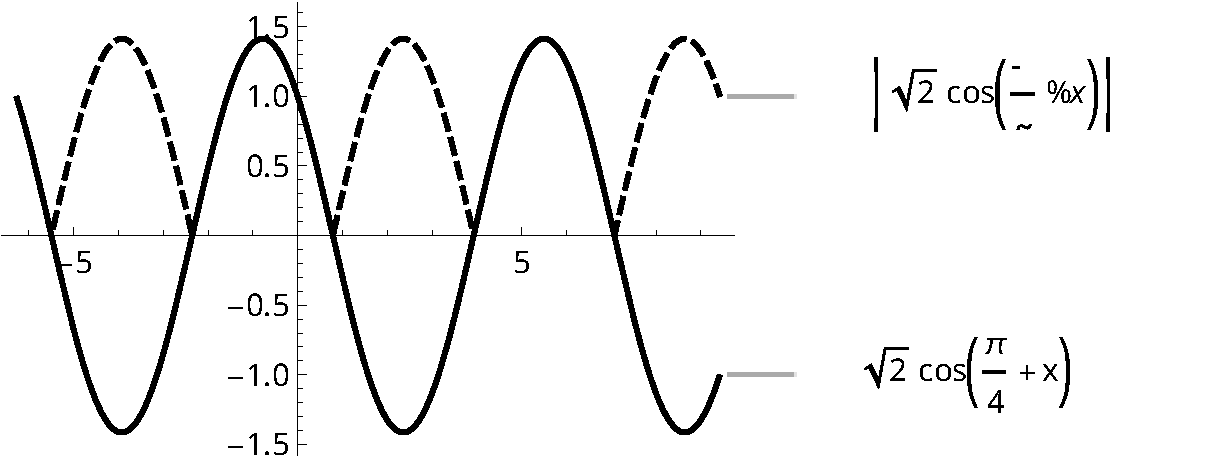
\includegraphics[width=0.5\textwidth]{figure/sqrt-2-cos-pi-slash-4-plus-x-with-without-abs.pdf}
    \caption{The figure of $\abs*{f}$ and $f$. This two function has been drawn overlapped over the $x$-axis.}
    \label{fig:sqrt-2-cos-pi-slash-4-plus-x-with-without-abs}
\end{figure}

\begin{figure}
    \centering
    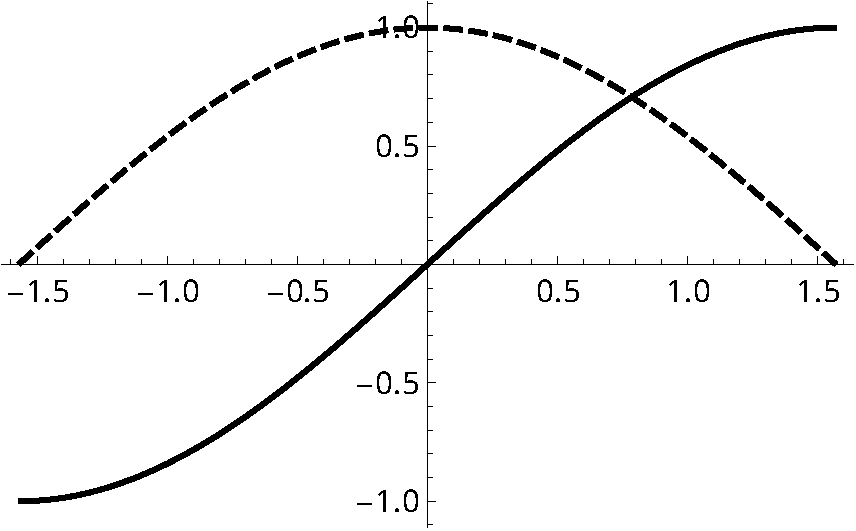
\includegraphics[width=0.5\textwidth]{figure/sin-and-cos-in-some-interval.pdf}
    \caption{The figure of $\sin x$(the solid curve) and it's deritative $\cos x$ on $[-\pi /2, \pi/2)$. }
    \label{fig:sin-and-cos-in-some-interval}
\end{figure}

\begin{example}
    \label{example:a-complicated-example-of-antiderivative-1}

    \cite[page 130]{yc}.
    \begin{align}
        \notag &\int \sqrt{1 - \sin 2x} \mathrm dx 
        \notag =\int \sqrt{1 - 2 \sin x \cos x} \mathrm dx \\
        \notag =&\int \sqrt{(\sin x + \cos x)^2} \mathrm dx 
        \notag =\int \abs*{\sin x + \cos x} \mathrm dx \\
        \label{eq:aux-angle-example-1} =&\int \underbrace{\abs*{\sqrt{2} \cos \left(x + \frac{\pi}{4}\right)}}_{f} \mathrm dx \\
        \label{eq:remove-abs-symbol-example-1} =
            & \underbrace{
                \left[
                    \splitfrac{
                        \overbrace{
                            \sqrt{2} \sin 
                            \left[(k + 1) \pi + \frac{\pi}{4} + x \right] 
                        }^{G}
                        + C_k,
                    }{
                        x \in \left[
                            k\pi + \frac{\pi}{4}, k \pi + \frac{5\pi}{4}
                        \right), k \in \mathbb Z 
                    }
                \right]
            }_{F}
    \end{align}
    由原函数在 $k\pi + \frac{5\pi}{4}$ 处的连续性
    \footnote{参见 Theorem \ref{thm:i-dont-know-how-to-name-this-theorem-2}}
    可知,
    \[
        C_{k + 1} = C_k + 2\sqrt{2}
    \]
    故原函数\footnote{如图 \ref{fig:a-complicated-antiderivative-example}}为
    \begin{align*}
        &\sqrt{2}\sin \overbrace{\left[(k+1) \pi + \frac{\pi}{4} + x\right]}^{A} + C + 2\sqrt{2} k \\
        &x\in \left[k\pi + \frac{\pi}{4}, k \pi + \frac{5\pi}{4}\right), k \in \mathbb Z 
    \end{align*}

    需要解释一下这个题,根据 FCM \footnote{Theorem \ref{thm:FCM}}
    式子 (\ref{eq:remove-abs-symbol-example-1}) 中 $f$ 要获得其原函数
    需要满足其绝对值的要求。
    若 $F$ 中不带有任何定义域限制,
    无法满足 $f$ 中绝对值的要求(如图 \ref{fig:sqrt-2-cos-pi-slash-4-plus-x-with-without-abs})。

    由式子 (\ref{eq:remove-abs-symbol-example-1}) 可得
    \[
        A \in \left[
            (2k + 1) \pi + \frac{\pi}{2}, (2k + 1) \pi + \frac{3\pi}{2}
        \right), k \in \mathbb Z
    \]
    进而可得\footnote{如图 (\ref{fig:sin-and-cos-in-some-interval}) 所示}
    \[
        \frac{\mathrm d}{\mathrm dx}\left(\sin A\right) \geq 0.
    \]
    综上,我们说明了对 $x$ 取值范围的限定,是为了保证式子 (\ref{eq:aux-angle-example-1})
    中的 $G' > 0$。

    \emph{连续函数的原函数必然连续},
    需要在原函数末添加一个特殊常量 $C_k$ 来满足。
    若不添加该常数,函数则为一带有周期跳跃间断点的函数,
    如图\ref{fig:a-complicated-antiderivative-example-wrong}所示。
\end{example}

上例通过直观的图像展示了题目各关键步骤的原因和其中的考虑。
对于做题来说,形如\footnote{$f$ 是周期函数}
\[
    F = \int \abs*{f(x)} \mathrm dx
\]
可理解为\emph{需要使 $F'(x) \geq 0$},换句话说就是需要 $F$ 是一个\emph{递增}函数。
\begin{enumerate}
    \item 使用一般方法解一个准原函数,
    \item 对自变量进行修改——通过仔细选取一个\emph{递增}的区间,并使用周期变量\footnote{上例中的 $k$}对其进行拓展。
    \item 之后在修饰后的\footnote{上例中$G$}原函数后加上一个周期相关的“常数”
        \footnote{
            上例中 $C_k$,我不知道周期相关的常数是否还可以被称之为常数。抑或者这是另一种分段函数的表现形式
        },使得原函数连续。
\end{enumerate}
其中第二部

\begin{figure}
    \centering
    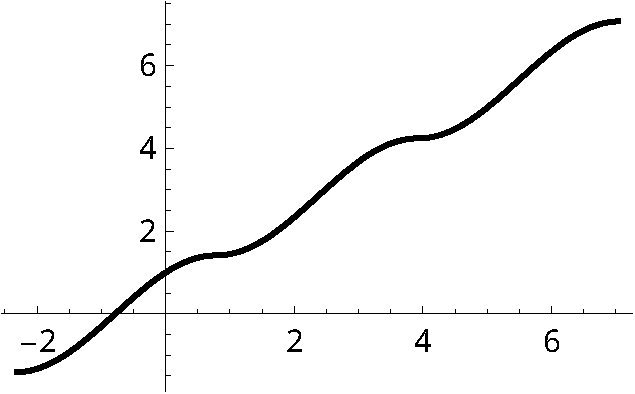
\includegraphics[width=0.5\textwidth]{figure/a-complicated-antiderivative-example.pdf}
    \caption{The figure of $F$ in Example \ref{example:a-complicated-example-of-antiderivative-1}. }
    \label{fig:a-complicated-antiderivative-example}
\end{figure}

\begin{figure}
    \centering
    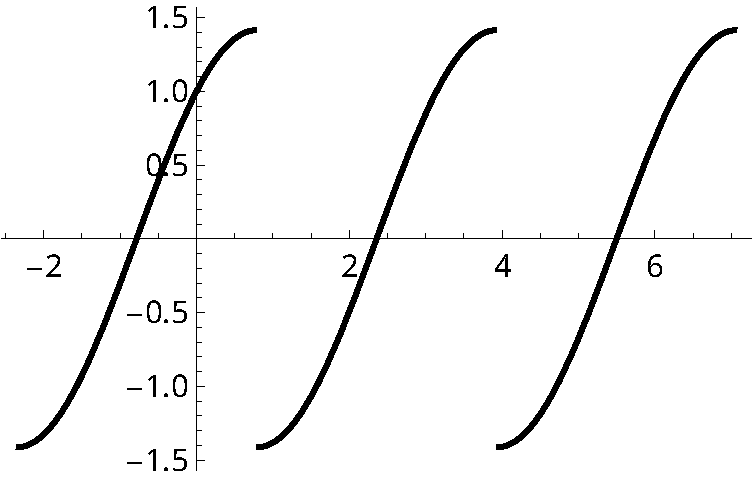
\includegraphics[width=0.5\textwidth]{figure/a-complicated-antiderivative-example-wrong.pdf}
    \caption{
        The figure of $G$ (equals $F - C_k$) 
        in Example
        \ref{example:a-complicated-example-of-antiderivative-1}. 
    }
    \label{fig:a-complicated-antiderivative-example-wrong}
\end{figure}

\subsection{两个概念的应用}

\begin{example}
    Let $f'(e^x) = \sin x$, what is the $f(x)$?

    \cite[page 101, example 1]{we}:

    本题目一方面可以通过令 $t = e^x$ 的方法然后进行比较常规的做法解出。
    另外还可以对等式两边同时对 $e^x$ 积,即:
    \[
        \int f'(e^x) \mbox{d} e^x = \int \sin x \mbox{d} e^x
    \]
    则 $\mbox{LHS} = f(e^x)$\footnote{应用了 FCM (Theorem \ref{thm:FCM}) part 1}, 
    $\mbox{RHS}$ 为一种很好的分部积分的形式。
    进一步解得 $f(e^x) = (e^x/2) (\sin x - \cos x) + C$ 后,
    再进行变量代换 $t = e^x$ 求出 $f(x)$ 即可。
\end{example}

\subsection{分部积分}\label{part-integral}

\begin{definition}
    Suppose both $u(x)$ and $v(x)$ has their one order continuous deritative repectively.
    Thus, 
    \[
        \int u \mbox{d} v = uv - \int v \mbox{d} u
    \]
\end{definition}

分部积分适用于 integrand 为两个不同类型函数的乘积时。
其中 $uv$ 的选择关系到做题速度,相关信息请参见 \cite[page 95, pdf 106]{we}.

\begin{example}
    \[
        \int x \sin x \mathrm dx
    \]

    \cite[page 486]{stewart}.

    \begin{gather*}
        u = x\quad \mathrm dv = \sin x \mathrm dx \\
        du = dx \quad v = -\cos x
    \end{gather*}
    and so
    \begin{align*}
        \int x \sin x \mathrm dx &= \int \overbrace{x}^{u} \overbrace{\sin x \mathrm dx}^{\mathrm dv} \\
                                 &= \underbrace{x}_{u}\underbrace{(-\cos x)}_{v} - \int \underbrace{(-\cos x)}_{v}  \underbrace{\mathrm dx}_{\mathrm du} \\
                                 &= -x \cos x + \int \cos x \mathrm dx \\
                                 &= -x \cos x + \sin x + C
    \end{align*}
\end{example}

\begin{example}
    \[
        \int e^x \sin x \mathrm dx
    \]

    \cite[page 488]{stewart}.

    Neither $e^x$ nor $\sin x$ becomes simpler when differentiated,
    so let's try choosing
    \footnote{It's turns out that, in this case, chosing $u = \sin x, \mathrm dv = e^x \mathrm dx$ also works.}
    $u = e^x$ and $\mathrm dv = \sin x \mathrm dx$. 
    Then $\mathrm du = e^x$ and $v = -\cos x$, so integration by parts gives
    \begin{equation}
        \label{eq:integration-by-part-example-eq2}
        \int e^x \sin x\mathrm dx = -e^x \cos x + \int e^x \cos x \mathrm dx
    \end{equation}
    The integral that we have obtained, $\int e^x \cos x \mathrm dx$, 
    is no simpler than the original one, but at least it's no more difficult.
     Having had success in the preceding example integrating
    by parts twice, we persevere and integrate by parts again. It is important that we again
    choose $u = e^x$, so $\mathrm dv = \cos x \mathrm dx$, 
    Then $\mathrm du = e^x \mathrm dx, v = \sin x$ and
    \begin{equation}
        \label{eq:integration-by-part-example-eq1}
        \int e^x \cos x \mathrm dx = e^x \sin x - \int e^x \sin x \mathrm dx
    \end{equation}
    At first glance, it appears as if we have accomplished nothing because we have arrived
    at $\int e^x \sin x \mathrm dx$, which is where we started, 
    However, if we put the expression for $\int e^x \mathrm dx$ 
    from Equation (\ref{eq:integration-by-part-example-eq1}) 
    into Equation (\ref{eq:integration-by-part-example-eq2}) 
    we get
    \begin{equation*}
        \int e^x \sin x \mathrm dx = -e^x \cos x + e^x \sin x - \int e^x \sin x \mathrm dx 
    \end{equation*}
    This can be regarded as an equation to be solved for the unknown integral. Adding
    $\int e^x \sin x\mathrm dx$ to both sides, we obtain
    \begin{align*}
        2 \int e^x \sin x \mathrm dx &= -e^x \cos x + e^x \sin x  \\
        \int e^x \sin x \mathrm dx &= \frac{1}{2} e^x (\sin x - \cos x) + C
    \end{align*}
\end{example}

定积分的分部积分法请参见小节 \ref{definite-integration-by-parts}.

\subsection{第一类换元法}

有理被积函数尤其是分式的时候,可以考虑 \textbf{加项减项拆}
的策略来将式子分为多个式子相加减的形式。
请参阅\cite[page 98, pdf 109, example 7]{we}

\subsection{第二类换元法}

\begin{table}
    \centering
    \begin{tabular}{cc}
        \toprule
        若式子中出现 & 令 \\
        \midrule
        $\sqrt{a^2 - x^2}$ & $x = a \sin t$或$x = a \cos t$ \\
        $\sqrt{a^2 + x^2}$ & $x = a \tan t$ \\
        $\sqrt{x^2 - a^2}$ & $x = a \sec t$ \\
        \bottomrule
    \end{tabular}
    \caption{常用第二类换元法替换}
    \label{tab:useful-sec-type-substitutions}
\end{table}
第二类换元法常用替换请参见表格 \ref{tab:useful-sec-type-substitutions}.

\subsection{三类常见可积函数中不熟悉的考点}

\subsubsection{三角有理积分}

即形如
\[
    \int R(\sin x, \cos x) \mbox{d} x 
\]
可以采用\textit{万能代换}法,令 $t = \tan (t/2)$, 则有
\begin{equation}
    \int R(\sin x, \cos x) \mbox{d} x 
    = \int R\left(\dfrac{2t}{1+t^2}, \dfrac{1-t^2}{1+t^2}\right) 
    \dfrac{2}{1+t^2} \mbox{d} x
\end{equation}
该方法虽然通用性很好,但是计算比较繁琐复杂
\footnote{若三角函数的次数为1,则可以考虑},
不到万不得已,不适用该方法。

\begin{table}
    \centering
    \begin{tabular}{ccc}
        \toprule
        若 & 令 \\
        \midrule
        $R(- \sin x,   \cos x) = -R(\sin x, \cos x)$ & $u = \cos x$ \\
        $R(  \sin x, - \cos x) = -R(\sin x, \cos x)$ & $u = \sin x$ \\
        $R(- \sin x, - \cos x) =  R(\sin x, \cos x)$ & $u = \tan x$ \\
        \bottomrule
    \end{tabular}
    \caption{常用三角有理式代换}
    \label{tab:useful-tri-rational-substitutions}
\end{table}
这种问题,最好先使用三角变形、换元、分部积分。
表\ref{tab:useful-tri-rational-substitutions}是常用的集中换元和其条件。

\subsubsection{简单无理积分} \label{simple-irrational-integral}

\begin{equation}
    \int R\left(x, \sqrt[n]{\dfrac{ax+b}{cx+d}}\right) \mathrm{d} x
\end{equation}
令 $\sqrt[n]{\dfrac{ax+b}{cx+d}}=t$ 将其化为有理函数进行计算。
\footnote{
    比\cite{we}更详细的讲解,请参见
    \url{https://zhuanlan.zhihu.com/p/413132173}.
}
\begin{align*}
    x &= \dfrac{d t^n-b}{a-c t^n} \\
    \mathrm{d} x &= \dfrac{n t^{n-1} (a d-b c)}{\left(a-c t^n\right)^2} \mathrm{d} t
\end{align*}
其中,若 $n = 1$
\begin{equation}
    \mathrm{d} x = \dfrac{ad-bc}{(a-ct)^2}
\end{equation}
若 $n = 2$
\begin{equation}
    \mathrm{d} x = \dfrac{2t(ad-bc)}{(a-ct^2)^2}
\end{equation}

\begin{example}
    求
    \[
        \int \dfrac{1}{x} \sqrt{\dfrac{x+1}{x}} \mathrm{d} x
    \]

    令 $t =\sqrt{\dfrac{x+1}{x}}$,则 $x = \dfrac{1}{t^2 - 1}$,
    $\mathrm{d}x = - \dfrac{2t}{(t^2 - 1)^2}$.
    则
    \begin{align*}
          &\int \dfrac{1}{x} \sqrt{\dfrac{x+1}{x}} \mathrm{d} x 
        = \int (t^2 - 1) t \dfrac{-2t}{(t^2-1)^2} \mathrm{d} t \\
        = &-2 \int \dfrac{t^2}{t^2-1} \mathrm{d} t
        = -2 \int \left(1+\dfrac{1}{t^2-1}\right) \mathrm{d} t\\
        = &-2\left(t + \dfrac{1}{2} \ln \left|\dfrac{t-1}{t+1}\right|\right) + \mathrm{C} \\
        = &-2 \sqrt{\frac{x + 1}{x}} - \ln \abs*{\frac{\sqrt{\frac{1+x}{x} }-1}{\sqrt{\frac{1+x}{x} } +1}} + \mathrm C
    \end{align*}
\end{example}

不要忘了不定积分换元后,结果要将符号换回去。

\subsection{分段函数的不定积分}

本题型考察的就是分段点的处理,只需保证积分后两个分段是连续的即可
\footnote{
    在考研数学中这种情况无需考生证明可导性,
    只需要说明分段被积函数\textbf{连续}即可
}。
参见 \cite[page 101, pdf 112, example 5]{we}.

\begin{example}
    求不定积分 $\int e ^{-|x|} \mathrm{d} x$

    \textbf{方法一:}
    \[
        e^{-|x|} = \left\{
            \begin{array}{rl}
                \mathrm{e} ^{-x} &, x \geq 0, \\
                \mathrm{e} ^x    &, x < 0.
            \end{array}
        \right.
    \]
    \[
        F(x) = \int \mathrm{e} ^{-|x|} \mathrm{d} x = \left\{
            \begin{array}{rl}
                - \mathrm{e} ^{-x} + \mathrm{C_1} &, x \geq 0, \\
                  \mathrm{e} ^x    + \mathrm{C_2} &, x < 0.
            \end{array}
        \right.
    \]

    \uline{
        $\mathrm{e}^{-|x|}$ 连续,
        原函数$F(x)$\textbf{必连续}, 从而$F(x)$
        在 $x = 0$ \textbf{连续}
    },由于
    \begin{align*}
        &\lim_{x \to 0^+} F(x) &= &\lim_{x \to 0^+}(-e^{-x} + C_{1})&=& -1& +\mathrm{C_{1}}  \\
        &\lim_{x \to 0^-} F(x) &= &\lim_{x \to 0^-}(e^{x} + C_{2})  &=&  1& +\mathrm{C_{2}} 
    \end{align*}
    所以 $ -1 + \mathrm{C_1} = 1 + \mathrm{C_2}$.
    \textbf{令 $C_1 = C$,则 $C_2 = -2 + C$} 因此
    \[
        \int \mathrm{e}^{-|x|} = \left\{
            \begin{array}{rl}
                - \mathrm{e}^{-x} + \mathrm{C} &, x \geq 0, \\
                  \mathrm{e}^{ x} - 2 + \mathrm{C} &, x < 0.
            \end{array}
        \right.
    \]

    \textbf{方法二:}
    由于 $\mathrm{e}^{-|x|}$ 连续,则$F(x) = \int_{0}^{x} \mathrm{e}^{-|x|} \mathrm{d} t$
    是其一个原函数,又
    \begin{align*}
        F(x) &= \int_{0}^{x} e^{-|t|} \mathrm{d} t = 
        \begin{dcases*}
            \cramped{\int_{0}^{x} \mathrm{e}^t    \mathrm{d} t} &, x < 0, \\
            \cramped{\int_{0}^{x} \mathrm{e}^{-t} \mathrm{d} t} &, x \geq 0.
        \end{dcases*}\\
        &= \begin{dcases*}
            \mathrm{e}^x - 1 &, x < 0 \\
            1 - \mathrm{e}^{-x} &, x \leq 0.
        \end{dcases*}
    \end{align*}
    \underline{则 $\int \mathrm{e}^{-|x|} \mathrm{d} x = F(x) + \mathrm{C}$}.
\end{example}
本例\footnote{注意下划线标记内容的表述方式。}
中,后一种不需要使用极限语言说明连续性,

\subsection{其它事项}

根据定义\ref{defination-definite-integral}可知,下列为不等式而非等式
\[
    \int \dfrac{f(x)}{g(x)} \mathrm{d}x 
    \neq 
    \dfrac{\int f(x) \mathrm{d} x}{\int g(x) \mathrm{d} x}
\]
Sigma 的使用注意事项请参见 \ref{giant-operator} 节。

\subsection{好题汇编}

\begin{example}
    求 $I_1 = \int \cos ^4 x \mathrm{d} x$, $I_2 = \int \sin ^4 x \mathrm{d} x$.
    \begin{align*}
        I_1 + I_2 &= \int 
                    \left[
                        (\sin ^2 x + \cos ^2 x)^2 - \dfrac{1}{2} \sin ^2 2x
                    \right] \mathrm{d}x \\
                  &= \int 1 - \dfrac{1}{2} \sin ^2 2x \mathrm{d} x \quad \mbox{(降幂很巧妙)}\\
                  &= \int 1 - \dfrac{1}{4} (1-\cos 4x) \mathrm{d} x \\
                  &= \dfrac{3}{4} x + \dfrac{1}{16} \sin x + C_1
    \end{align*}
    \begin{align}
        I_1 - I_2 &= \int \cos ^4 x - \sin ^4 x \mathrm{d}x \notag \\
                  &= \int \cos 2x \mathrm{d}x \label{eq:app-trig-double-angle-1} \\
                  &= \dfrac{1}{2} \sin 2x +C_2 \notag
    \end{align}
    所以
    \begin{align*}
        I_1 &= \dfrac{1}{2} \left[(I_1+I_2)+(I_1-I_2)\right] \\
            &= \frac{3}{8} x + \frac{1}{32} \sin 4x + \frac{1}{4} \sin 2x + C_1 \\
        I_2 &= \dfrac{1}{2} \left[(I_1+I_2)-(I_1-I_2)\right] \\
            &= \frac{3}{8} x + \frac{1}{32} \sin 4x - \frac{1}{4} \sin 2x + C_2
    \end{align*}
    \cite[page 26, question 57]{w660ans}
\end{example}
上例巧妙利用积分的和等于和的积分这一性质,将两个积分组合到一起。
这样更便于使用初等数学中三角恒等变换的知识辅助解题。

式子 (\ref{eq:app-trig-double-angle-1}) 利用了三角函数二倍角公式。
三角函数相关公式请参见小节 \ref{trigonometric}.

\section{定积分}\label{finite-integral}

\subsection{定积分的概念}\label{concept-of-definite-integral}

\begin{itemize}
    \item 定积分概念
    \item 定积分几何意义
    \item 可积性
    \item \textbf{计算(重点)}
    \item \textbf{变上限积分(重点)}
    \item 定积分性质
    \item \underline{积分不等式(难点)}
\end{itemize}

使用黎曼和定义,根据几何意义的细微差别解析式形式也有细微不同,
但他们的值都是相同的:
\begin{definition}[Definite Integral]\label{defination-definite-integral}
    If $f$ is a fuction defined for $a \leq x \leq b$, 
    we devide the interval $[a, b]$ into $n$ subintervals of equal width
    $\Delta x = (b - a) / n$.
    We let $x_0 (=a), x_1, x_2, x_3, \cdots, x_n (=b)$ be the endpoints
    of these subintervals and we let $x_1^*, x_2^*, \cdots, x_n^*$ 
    be any \textbf{sample points} in these subintervals, so $x_u^*$
    lies in the $i$th subinterval $[x_{i-1}, x_i]$.
    Then the \textbf{definite integral of $f$ from $a$ to $b$} is
    \[
        \int_{a}^{b} f(x) \mbox{d} x = 
        \lim_{n \to \infty} \sum_{i = 1}^{n} f\left(x_i^*\right) \Delta x
    \]
    provided that this \emph{limit exists} 
    and gives the same value for all
    possible choices of sample point. 
    \emph{If it does exist, we say that 
    $f$ is \textbf{integrable} on $[a, b]$}.
    \cite[page 384]{stewart}
\end{definition}
上述定义式中 $\Delta x$ 可以写作 $\dfrac{1}{n}$
\footnote{被武忠祥老师称为“可爱因子”}, 
$x^*_i$ 可以写作 $\dfrac{i}{n}$, 
这样式子就变成了
\begin{equation}\label{eq:the-other-definition-definite-integral}
    \lim_{n \to \infty} \dfrac{1}{n}
    \sum_{i = 1}^{n} \underbrace{f\left(\dfrac{i}{n}\right)}_{\mathclap{\mbox{\small 右端点函数值}}} 
\end{equation}
\begin{equation}
    \lim_{n \to \infty} \dfrac{1}{n}
    \sum_{i = 1}^{n} \underbrace{f\left(\dfrac{i-1}{n}\right)}_{\mathclap{\mbox{\small 左端点函数值}}}
\end{equation}
\begin{equation}
    \lim_{n \to \infty} \dfrac{1}{n}
    \sum_{i = 1}^{n} \underbrace{f\left(\dfrac{2i-1}{2n}\right)}_{\mathclap{\mbox{\small 中点函数值}}} 
\end{equation}
上述三个公式是完全等价的。

\subsection{存在性}
\begin{align}
    f(x) \mbox{\small 可积} &\quad         \Longrightarrow  \quad f(x) \mbox{\small 有界} \\
    f(x) \mbox{\small 有界} &\quad \cancel{\Longrightarrow} \quad f(x) \mbox{\small 可积} \notag
\end{align}

\begin{theorem}[Integrable Theorem] \label{integrable-therom}
    If $f$ \underline{is continuous on $[a,b]$},
    or if $f$ has only 
    \underline{a finite number of \textit{jump discontinuities}}
    \footnote{按照武忠祥老师的说法,这里第一类间断点也可(跳跃、可去)}, 
    then $f$ is \emph{integrable} on $[a, b]$;
    that is, the definite integral $\int_a^b f(x) \mathrm{d} x$ exists.
\end{theorem}

\begin{align}
    f(x) \mbox{\small 连续} &\quad         \Longrightarrow  \quad f(x) \mbox{\small 可积} \\
    f(x) \mbox{\small 可积} &\quad \cancel{\Longrightarrow} \quad f(x) \mbox{\small 连续} \notag
\end{align}

\begin{example}
    设
    \[
        f(x) = 
        \begin{dcases*}
            \sin \frac{1}{x}, & x \neq 0 \\
            1, & x = 0
        \end{dcases*}, 
        F(x) = \int_{-1}^{x} f(t) \mathrm dt
    \]
    则 $F(x)$ 
    \begin{itemize}
        \item[A] 在 $(-1, 1)$ 为无界函数
        \item[B] 在 $(-1, 1)$ 为连续有界函数
        \item[C] 在 $(-1, 1)$ 有间断点 $x = 0$
        \item[D] 在 $[-1, 1]$ 不可积
    \end{itemize}
    
    \cite[question 177]{w660}.

    $f(x)$ 在 $[-1, 1]$ 有界,只有一个间断点 $x = 0$,
    那么 $f(x)$ 在 $[-1, 1]$ 可积,
    继而 $F(x)$ 在 $[-1, 1]$ 连续,所以有界。选择B.
\end{example}

\begin{example}
    下列命题中正确的是
    \begin{itemize}
        \item[A] 设 $f(x)$ 在 $[a, b]$ 可积,$f(x) \leq 0, \nequiv 0, $ 则
            \[
                \int_a^b f(x) \mathrm dx > 0
            \]
        \item[B] 设 $f(x)$ 在 $[a, b]$ 可积,$g(x)$ 在 $[a, b]$ 不可积,则 $f(x) + g(x)$ 在 $[a, b]$ 不可积。
        \item[C] 设 $f^2(x)$ 在 $[a, b]$ 可积,则$f(x)$ 在 $[a, b]$ 可积
        \item[D] 设 $x_0 \in (a, b), f(x)$ 在 $[a, b]\textbackslash \{x_0\}$ 连续且有界,
            $x = x_0$ 是 $f(x)$ 的间断点,则
            \[
                F(x) = \int_a^x f(t) \mathrm dt
            \]
            在 $x = x_0$ 不可导
    \end{itemize}

    \cite[question 181]{w660}.

    选项B是正确的,体现了 linearinity.
    若 $f(x) + g(x)$ 在 $[a, b]$ 可积,因 $f(x)$ 在 $[a, b]$ 上可积,
    由 linearinity 可知,
    \[
        g(x) = [f(x) + g(x)] - f(x)
    \]
    在 $[a, b]$ 可积,与已知 $g(x)$ 在 $[a, b]$ 上不可积矛盾,
    因此 $f(x) + g(x)$ 在 $[a, b]$ 上不可积
\end{example}

\subsection{定积分计算}

\subsection{分部积分(定积分)}
\label{definite-integration-by-parts}

\begin{definition}
    \textbf{Assuming $f'$ and $g'$ are continuous on $[a, b]$}, 
    and using the Fundamental Theorem, we obtain
    \[
        \int_a^b f(x) g'(x) \mathrm dx = \left. f(x)g(x) \right]_a^b - \int_a^b g(x)f'(x) \mathrm dx
    \]
\end{definition}

\subsubsection{公式}

周期性定积分公式:
\begin{lemma}
    \begin{equation}
        \int_a^{a + T} f(x) \mathrm{d} x = \int_0^T f(x) \mathrm{d} x
    \end{equation}
\end{lemma}

三角函数有关的公式:
\begin{lemma}[点火公式]
    \begin{multline}\label{eq:launching-formula}
        \int_0^{\frac{\pi}{2}} \sin ^n x \mathrm{d} x = \int_0^{\frac{\pi}{2}} \cos ^n x \mathrm{d} x \\
        = 
        \left\{ 
            \begin{array}{rl}
                \dfrac{n - 1}{n} \cdot \dfrac{n - 3}{n - 2} \cdot \cdots \cdot \dfrac{1}{2} \cdot \dfrac{\pi}{2} &, n \mbox{\small \ is even.}   \\[1em]
                \dfrac{n - 1}{n} \cdot \dfrac{n - 3}{n - 2} \cdot \cdots \cdot \dfrac{2}{3}                      &, n \mbox{\small \ is odd} > 1 \\
            \end{array}
        \right.
    \end{multline}
    
    若 $f(x)$ 连续,则
    \begin{equation}
        \label{eq:magic-trig-integration-simplification-1}
        \int_0^{\pi} x f(\sin x) \mathrm{d} x = \dfrac{\pi}{2} \int_0^{\pi} f(\sin x) \mathrm{d} x
    \end{equation}
\end{lemma}

\begin{example}
    \[
        I = \int_0^{\pi} x \sqrt{\cos^2 x - \cos^4 x} \mathrm dx
    \]

    \cite[question 187]{w660}.

    由公式 (\ref{eq:magic-trig-integration-simplification-1}) 得
    TODO %TODO
\end{example}

\section{广义积分中值定理} 

\begin{theorem}[广义积分中值定理] 
    \label{general-mean-value-theorm-of-integral}
    若 $f(x), g(x)$ 在 $[a, b]$ 上连续,且 $g(x)$ 不变号,则
    \begin{equation}
        \label{eq:general-mean-value-theorm-of-integral-equation}
        \int_a^b f(x) g(x) \mathrm{d} x = 
        f(\xi) \int_a^b g(x) \mathrm{d} x,\ \underline{a \leq \xi \leq b}.
    \end{equation}
    当取 $g(x) = 1$ 则有
    \begin{equation}
        \label{eq:non-general-mean-value-theorm-of-integral-equation}
        \int_a^b f(x) \mathrm{d} x = 
        f(\xi)(b - a),\  \underline{a < \xi < b}
        \quad
        \footnote{
            这里的不等号仅可用于考研。
            欲对数学进行更深层次了解,请参考数学分析教程。
        }.
    \end{equation}
    后者可直接用拉格朗日中值定理\footnote{参见\ref{thm:lagrange}}证明。
\end{theorem}
另外,若被积函数和参数有关,即形如$f(x, t)$的,上面式子中的 $\xi$
也将会和 $t$ 相关,不同的 $t$,可能会造成不同的 $\xi$。
比如 \cite[page 106, pdf 117, example 3]{we}。
还可参考例子 \ref{example-limits-and-varidic-limits-integral-2} 和下例。
\begin{example}
    设 $f(x)$ 为连续函数,
    \[
        g(x) = \int_{-x}^{0} t f(x + t) \mathrm dt
    \]
    则 $g'(x) =$ 

    \cite[question 155]{w660}.
    
    令 $u = x + t$, 则有
    \begin{align*}
        g(x) &= \int_{-x}^0 tf(x + t) \mathrm dt = \int_0^x (u - x) f(u) \mathrm du \\
             &= \int_0^x uf(u) \mathrm du - x \int_0^x f(u) \mathrm du
    \end{align*}
    则
    \[
        g'(x) = xf(x) - \int_0^x f(u) \mathrm du - xf(x) = - \int_0^x f(u)
    \]
\end{example}

\begin{example}
    设 $f(x)$ 一阶可导,$f(x) > 0, f'(x) > 0$,
    则当 $\Delta x > 0$ 时
    \begin{itemize}
        \item[A] \[\int_{x}^{x + \Delta x} f(t) \mathrm dt > f(x)\Delta x > 0\]
        \item[B] \[f(x)\Delta x >\int_{x}^{x + \Delta x} f(t) \mathrm dt > 0\]
    \end{itemize}
    
    \cite[question 178]{w660}.

    \begin{align*}
        &\int_x^{x + \Delta x} 
        f(t) \mathrm dt \\
        \xrightarrow[=]{\mbox{\small 中值定理}} 
        &f(\xi) [(x + \Delta) - x], \quad \xi \in (x, x + \Delta x) \\
        =&f(\xi) \Delta x > f(x) \Delta x
    \end{align*}

    所以选A.
\end{example}

\section{和定积分有关的极限问题} 
\label{limit-questions-involved-definite-integral}

题型有三种:
\begin{itemize}
    \item 用定积分定义
          \footnote{Definition \ref{defination-definite-integral}}
          求极限
          \footnote{另请参见\ref{use-squeeze-or-definition-of-integral}节}
    \item 积分上下限之差是常数
        \begin{itemize}
            \item 积分中值定理(Section
                \ref{general-mean-value-theorm-of-integral})
        \end{itemize}
    \item 积分上下限不变,极限变量在被积函数上
        \begin{itemize}
            \item 夹迫定理
            \item 积分中值定理(Section
                \ref{general-mean-value-theorm-of-integral})
        \end{itemize}
\end{itemize}

\begin{example}
    设 $f(x)$ 连续,且 \[\lim_{x \to +\infty} f(x) = 1\]
    则 \[\lim_{x \to +\infty} \int_x^{x+2} t \sin\left(\frac{3}{t}\right)f(t) \mathrm dt\] 是多少?
    \cite[page 106, pdf 117]{we}

    积分的上下限之差为一个常数,即 \[(x + 2) - x = 2\]
    这种题型一般就可以选用
    \emph{积分中值定理}
    \footnote{
        本例使用的是非广义积分中值定理
        (式子\ref{eq:non-general-mean-value-theorm-of-integral-equation})
    } 来处理。
    \begin{align*} 
         &\lim_{x \to +\infty} \int_x^{x+2} t \sin\left(\frac{3}{t}\right)f(t) \mathrm{d} t\\
        =&\lim_{x \to +\infty} 2 \xi \sin \left(\dfrac{3}{\xi}\right) f(\xi) \quad \underline{(x < \xi < x+2)}\\
        =&\lim_{\xi \to +\infty} 2 \xi \sin \left(\dfrac{3}{\xi}\right) \\
        =&\lim_{t \to 0} 2 \cdot \frac{\sin 3t}{t} \quad \mbox{\small (等价无穷小代换)}\\ 
        =&\lim_{t \to 0} 2 \times 3 \\
        =&6
    \end{align*}
    取值范围声明(下划线部分)不要忘了写!
\end{example}

\begin{example}
    求极限
    \[
        \lim_{x \to \infty} \int_0^1 x^n \sqrt{1+x^2} \mathrm{d}x
    \]
    \cite[page 106, pdf 117]{we}

    \begin{align*}
        &0 \leq \int_0^1 x^n \sqrt{1+x^2} \mathrm{d}x 
        < \underbrace{\sqrt{2} \int_0^1 x^n 
        \mathrm{d}x}_{\mbox{\small 定积分性质}} \\
        &= \dfrac{\sqrt{2}}{n+1}
    \end{align*}
    又\footnote{the Squeeze Theorem}
    \[
        \lim_{x\to \infty} \dfrac{\sqrt{2}}{n+1} = 0
    \]
    所以 $\mbox{LHS} = 0$.
\end{example}
有时候有可能会想要将极限拿到积分里面先进行运算,
这种做法是否合理已经超纲,所以这个办法不能用。
但是可以用于辅助分析该极限的值,进而转用其他
大纲以内的知识,比如夹迫定理来求值。

应用\emph{放缩法}来凑夹迫定理条件的时候
\[
    \int_0^1 x^n \sqrt{1+x^2} \mathrm{d}x
\]
式子中 $\sqrt{1+{x^{*}_{i}}^2}$ 最大为 $\sqrt{2}$
\footnote{
    ${x^{*}_{i}}$可以看作$\frac{i}{n}$,
    更多信息参见\ref{concept-of-definite-integral}小节
},因此将它提出来,
之后剩下的 $\int_0^1 x^n \mathrm{d}x$ 可以直接计算出来也就是$1/(n+1)$。

另外,若要使用积分中值定理来解题要千万注意。
对被积函数来说,式子中的$t$是一个参数,得到的$\xi$依赖该参数的值。

%TODO

\section{定积分计算(公式)}

\begin{figure}
    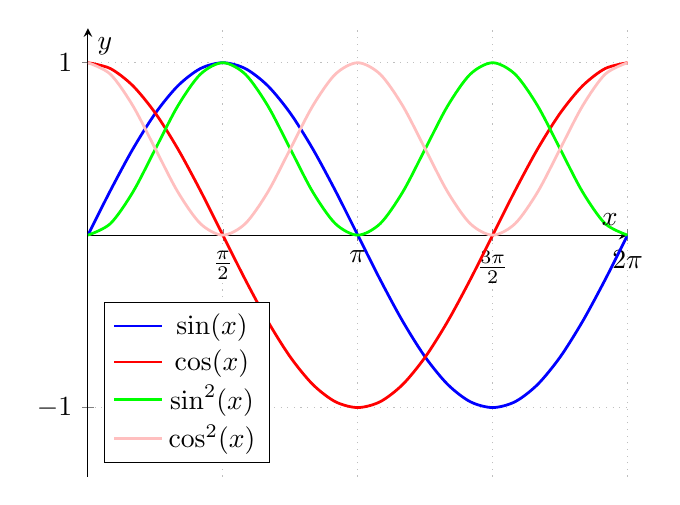
\begin{tikzpicture}
        \begin{axis}[
            domain=0:2*pi,  % Adjusted domain to [0, 2*pi]
            xmin=0, xmax=2*pi,
            ymin=-1.4, ymax=1.2,
            axis lines=middle,
            xlabel={$x$},
            ylabel={$y$},
            xtick={0,1.5708,3.1416,4.7124,6.2832},  % Adjusted xticks for [0, 2*pi]
            xticklabels={$0$,$\frac{\pi}{2}$,$\pi$,$\frac{3\pi}{2}$,$2\pi$},  % Adjusted xtick labels
            ytick={-1,0,1},
            legend pos=south west,
            grid=both,
            grid style={dotted},
        ]

        % Plot sine function
        \addplot[blue,smooth, line width = 1pt] {sin(deg(x))};
        \addlegendentry{$\sin(x)$};

        % Plot cosine function
        \addplot[red,smooth, line width = 1pt] {cos(deg(x))};
        \addlegendentry{$\cos(x)$};

        % Plot sine function
        \addplot[green,smooth, line width = 1pt] {(sin(deg(x)))^2};
        \addlegendentry{$\sin^2(x)$};

        % Plot cosine function
        \addplot[pink,smooth, line width = 1pt] {(cos(deg(x)))^2};
        \addlegendentry{$\cos^2(x)$};

        \end{axis}
    \end{tikzpicture}
    \caption{Sine 和 Cosine 函数在 $[0, 2\pi]$ 的图像}
    \label{fig:sin-and-cos-in-0topi}
\end{figure}

由图\ref{fig:sin-and-cos-in-0topi}
可以归纳出,在区间 $[0,\pi]$ 上三角函数的对称性。
进而可以帮助简化积分的计算。

\subsection{和圆有关的}
\label{definite-integral-about-circle-area}

利用定积分几何意义可知:
\begin{align}
    \int_0^{a}  \sqrt{a^2 - x^2} \mathrm dx &= \dfrac{\pi}{4} a^2 \quad,(a > 0) \label{eq:unit-circle-1-for-integral-evaluation}\\
    \int_0^{a}  \sqrt{2ax - x^2} \mathrm dx &= \dfrac{\pi}{4} a^2 \quad,(a > 0) \label{eq:unit-circle-2-for-integral-evaluation}\\
    \int_0^{2a} \sqrt{2ax - x^2} \mathrm dx &= \dfrac{\pi}{2} a^2 \quad,(a > 0) \label{eq:unit-circle-3-for-integral-evaluation}
\end{align}
其中,
\begin{itemize}
    \item 公式\ref{eq:unit-circle-1-for-integral-evaluation}是一个圆心在$(0, 0)$上的,半径为 $a$ 的$(1/4)$圆的面积;
    \item 公式\ref{eq:unit-circle-2-for-integral-evaluation}是一个圆心在$(a, 0)$上的,半径为 $a$ 的$(1/4)$圆的面积;
    \item 公式\ref{eq:unit-circle-3-for-integral-evaluation}是一个圆心在$(a, 0)$上的,半径为 $a$ 的$(1/2)$圆的面积;
\end{itemize}
% TODO 用 tikz 绘制几个示意图应该效果更好

\subsection{和三角函数奇偶性有关的}

\begin{align}
    \int_0^{\pi} \sin^n x \mathrm{d}x &= 2 \int_0^{\pi/2} \sin^n x \mathrm{d}x \\
    \int_0^{\pi} \cos^n x \mathrm{d}x &= 
    \left\{
        \begin{array}{rl}
            0,                                       &n \mbox{\small \ is odd} \\
            2 \int_{0}^{\pi/2} \cos^n x \mathrm{d}x, &n \mbox{\small \ is even}
        \end{array}
    \right.
\end{align}
这两个公式要结合函数的奇偶性和图像进行深入了解,参见图 
\ref{fig:sin-and-cos-in-0topi}.
两个公式右侧可进一步使用公式\ref{eq:launching-formula}进行求值。
例题参见 \cite[page 108, pdf 119, exmaple 3]{we}.

\subsection{三角函数的线性组合之比的积分}

即形如:
\[
    I = \int \dfrac{a \sin x + b \cos x}{c \sin x + d \cos x}\mathrm{d}x
\]
的,可用下面的待定系数方法简化运算
\begin{equation}
    I = \int 
    \dfrac{
         A(\overbrace{c \cos x - d \sin x}^{\mbox{\small 分母的导数}})
        +B(\overbrace{c \sin x + d \cos x}^{\mbox{\small 分母}})
    }{c \sin x + d \cos x} \mathrm{d}x
\end{equation}
其中$A, B$可以通过令两个分子相等解出。
参见\cite[page 110, pdf 121, example 8]{we}.

\subsection{积分上下限重现换元法}
\label{integral-limits-regenerating-substituting}

这个办法就是通过巧妙地选取换元变量,
是的换元前后的定积分上下限不变,
这样就有
\[
    I = \int_a^b f_1(x) \mathrm{d}x = \int_a^b f_2(t) \mathrm{d}t
\]
其中 $f_2(t)$ 是换元之后的 $f_1(x)$, $x = a + b - t$。
则
\[
    I = \dfrac{1}{2} \int_a^b 
    \underbrace{f_1(x) + f_2(x)}_{{\mbox{\small 这里可以消去一些麻烦}}}
    \mathrm{d}x
\]
只在原函数很难找到的使用,不是万金油。
另外对于多元函数积分利用该方法之前要先用被积函数变量对称性来对积分进行处理,
请参考小节\ref{multivariable-integral-properity-of-variable-symtric}.

参见\cite[page 110, pdf 121, example 8]{we}.

\begin{example}
    \[
        I = \int_0^{\pi} \dfrac{x |\sin x \cos x|}{1+\cos^2 x} \mathrm{d}X
    \]
    \cite[question 64]{w660}
\end{example}

另外还有一种类似的pattern也适合本方法。
令 $x = -x$
\[
    I = \int_{-a}^{a} f(x) \mathrm{d}x = \int_{-a}^{a} f(-t) \mathrm{d}t
\]
得到
\[
    2I = \int_{-a}^{a} \left[f(x) + f(-x)\right] \mathrm{d}x
\]

\subsection{关于 x 的边上限积分等式,求f(x)的定积分}
\begin{enumerate}
    \item 等式两边求导得到关系式
        \begin{itemize}
            \item 有参数在被积函数中存在形式形如$xf(x - t)$的,
                  首先进行换元,
                  使得被积函数转换为形如$(x - u)f(u)$的形式,
            \item 然后再进行拆项求积分
        \end{itemize}
    \item 带点进去关系式
\end{enumerate}

\begin{example}
    \[
        I = \int _0^{\pi/2} \dfrac{\sin x}{\sin x + \cos x} \mathrm{d}x 
    \]
    \cite[page 111, pdf 122, example 10]{we}.

    令 $x = \frac{\pi}{2} + 0 - t$, $\mathrm{d}t = -t$
    \footnote{这里的积分上下限应当倒转,但是有一个 $-1$ 直接又给倒回来了。}

    \begin{align*}
        &\int_0^{\pi/2} \dfrac{\sin x}{\sin x + \cos x} \mathrm{d}x 
        = \int_0^{\pi/2} \dfrac{\cos t}{\sin t + \cos t} \mathrm{d}t \\ 
        = &\dfrac{1}{2} 
        \left(
            \int_0^{\frac{\pi}{2}} 
            \dfrac{\sin x}{\sin x + \cos x} \mathrm{d}x 
            + \int_0^{\frac{\pi}{2}} 
            \dfrac{\cos x}{\sin x + \cos x} \mathrm{d}x
        \right) \\
        = &\dfrac{1}{2} \int_0^{\pi/2} \mathrm{d}x = \dfrac{\pi}{4}
    \end{align*}
\end{example}

\subsection{累次积分计算}

\begin{definition}[累次积分交换次序]
    \begin{align*}
         &\int_a^b \mathrm{d}x \int_{\phi_1(y)}^{\phi_2(y)} 
         f(x, y) \mathrm{d}y \\[1em]
        =&\int_a^b
        \left[
            \int_{\phi_1(y)}^{\phi_2(y)} f(x, y) \mathrm{d}y
        \right] \mathrm{d}x
    \end{align*}
\end{definition}

\begin{example}
    计算二次积分$\int_0^1 \mathrm{d}x \int_{x^2}^{x} xy^2 \mathrm{d}y$
    \begin{align*} 
        &\int_{0}^{1} \text{d}x \int_{x^2}^{x} xy^2 \text{d}y  \\
        = &\int_{0}^{1} 
        \left[ 
            \int_{x^2}^{x} xy^2 \text{d}y 
        \right] 
        \text{d}x 
        = \int_{0}^{1} 
        \left[ 
            \frac{xy^3}{3} 
        \right]_{x^2}^{x} \text{d}x \\ 
        =& \frac{1}{3} \int_{0}^{1} (x^4 - x^7) \text{d}x 
        = \frac{1}{3} 
        \left[ 
            \frac{x^5}{5} - \frac{x^8}{8} 
        \right]_{0}^{1} \\ 
        =& \frac{1}{3} \cdot \frac{3}{40} = \frac{1}{40}.
    \end{align*}

    \url{https://www.zhihu.com/question/517593800}
\end{example}

\subsection{例题}

\begin{example}\label{example:w660t60}
    \[
        I = \int_0^1 \left(\sqrt{\underbrace{2x-x^2}_{-(x-1)^2\mbox{\small 的一部分}}} 
        - \underbrace{\sqrt{(1-x^2)^3}}_{\mbox{\small 出现}\sqrt{a^2-x^2}\mbox{\small 形}}\right) \mathrm{d}x
    \]

    \cite[page 24, question 60]{w660}

    上面第二个大括号提示请参见表 \ref{tab:useful-sec-type-substitutions}.
    按照表中提示,令 $x = \sin t$,那么
    \begin{align*}
        \int_0^1 \left(
            \sqrt{(1-x^2)^3}
        \right) \mathrm{d}x
        &=
        \int_0^1 
            \cos^4 x
        \mathrm{d}x\\
        &=
        \frac{3}{4} \times \frac{1}{2} \times \frac{\pi}{2} = \frac{3}{16} \pi
    \end{align*}
    之后可运用点火公式 \ref{eq:launching-formula} 计算高次幂三角函数。

    式子中的前面一部分的化简目标为单位元面积,
    参见小节 \ref{definite-integral-about-circle-area}。
    则令 \[t = (x-1)\] 则 $2x-x^2 = 1-t^2$
    \[
        \int_0^1 \sqrt{2x-x^2} \mathrm{d}x
        = 
        \int_{-1}^0 \sqrt{1-t^2} \mathrm{d}t = \frac{\pi}{4}
    \]
    
    那么 \[I = \dfrac{\pi}{4} - \dfrac{3\pi}{16} = \dfrac{\pi}{16}\]
\end{example}

\begin{example}
    \[
        I = \int_0^1 \arcsin x \cdot \arccos x \mathrm{d}x
    \]
    \cite[page 24, question 59]{w660}
    一个方法是代换 $t = \arcsin x$ 之后进行分部积分。

    另外一个方法是直接对$I$进行分部积分。可以得到
    \begin{align*}
        I &= \left. \arccos x \arcsin x \right|^{1}_{0} 
             - \int_0^1 x \mathrm{d} \arcsin x \arccos x \\
          &= - \int_0^1 x 
          \left(
              \dfrac{\arccos x}{\sqrt{1-x^2}} 
              - \dfrac{\arcsin x}{\sqrt{1-x^2}}
          \right)
          \mathrm{d}x \\
          &= - 
          \left(
              \underbrace{
                  \int_0^1
                      \dfrac{\arccos x}{\sqrt{1-x^2}} \cdot x
                  \mathrm{d}x 
              }_{A}
              -
              \underbrace{
                  \int_0^1
                      \dfrac{\arcsin x}{\sqrt{1-x^2}} \cdot x
                  \mathrm{d}x 
              }_{B}
          \right) \\[1em]
        A &= - \int_0^1 \arccos x \, \mathrm{d} \sqrt{1-x^2} \\
          &= \left.- \arccos x \sqrt{1-x^2}\right]_0^1 + \int_0^1 \sqrt{1-x^2} \cdot 
              \dfrac{-\mathrm{d}x}{\sqrt{1-x^2}} \\
          &= - \dfrac{\pi}{2} + 1 
    \end{align*}
    同理可得 $B = 1, I = -\dfrac{\pi}{2} + 2$.
\end{example}

\begin{example}
    \[
        I = \int \dfrac{1}{1+\cos x} \mathrm{d}x 
          = \dfrac{1}{2} \int \sec^2 \dfrac{t}{2} \mathrm{d}t
    \]
\end{example}

\begin{example}
    \[
        I = \int_0^{\pi/2} \dfrac{1}{(\sin x + \cos x)^2} \mathrm{d}x
    \]

    Solution1:
    \begin{align*}
        I &= \int_0^{\pi/2} \dfrac{1}{1 + \sin 2x} \mathrm{d}x\\
          &= \dfrac{1}{2} \int_{0}^{\pi} \dfrac{1}{1+\sin x} \mathrm{d}x\\
          &= \dfrac{1}{2} \int_{\pi/2}^{\pi + \pi/2} \dfrac{1}{1+\cos x} \mathrm{d}x \quad (\mbox{\small 诱导公式})\\
          &\mbox{D.N.E}
    \end{align*}
    该解法无法求得定积分,因为被积函数在积分区间上有无穷间断点。如下图所示
    \begin{figure}[H]
        \centering
        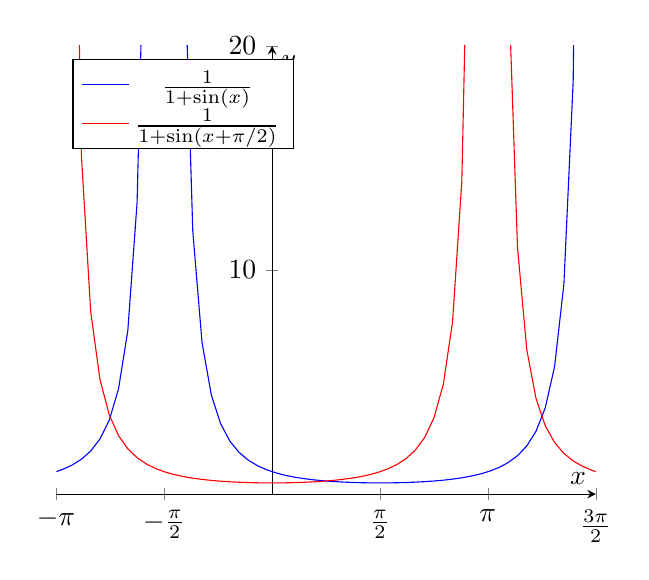
\begin{tikzpicture}
            \begin{axis}[
                axis lines=middle,
                xlabel={$x$},
                ylabel={$y$},
                xmin=-pi,
                xmax=3*pi/2,
                ymin=0,
                ymax=20,
                xtick={-pi,-pi/2,0,pi/2,pi,3*pi/2},
                xticklabels={$-\pi$,$-\frac{\pi}{2}$,$0$,$\frac{\pi}{2}$,$\pi$,$\frac{3\pi}{2}$},
                ytick={0,10,20},
                legend pos= north west,
                domain=-270:270, % Use degrees instead of radians
                restrict y to domain = 0:1000,
                samples=4000,    % Increase the number of samples for smoothness
            ]

            % Function 1
            \addplot[blue] {1/(1 + sin(deg(x)))};
            \addlegendentry{$\frac{1}{1 + \sin(x)}$}

            % Function 2
            \addplot[red] {1/(1 + sin(deg(x) + 90))}; % 90 degrees is equivalent to pi/2 radians
            \addlegendentry{$\frac{1}{1 + \sin(x + \pi/2)}$}

            \end{axis}
        \end{tikzpicture}
    \end{figure}
    所以在凑微分 $\sec^2 x$ 的时候要注意积分区间内是否出现无穷间断点。

    Solution2:
    \begin{align*}
        I &= \int_0^{\pi /2} \dfrac{1}{\left[\sqrt{2} \sin \left(x+\dfrac{\pi}{4}\right)\right]^2} \mathrm{d}x \\
          &= \dfrac{1}{2} \int_0^{\pi/2} \sec^2 \left(x-\dfrac{\pi}{4}\right)\mathrm{d} x-\dfrac{\pi}{4}\\
          &= \left. \dfrac{1}{2} \tan \left(x - \dfrac{\pi}{4}\right) \right]^{\pi/2}_{0}
    \end{align*}
    解法2应用了辅助角公式,但是在这里,并没有体现辅助角。
\end{example}

\section{变上限积分积分及其应用}

考点:
\begin{itemize}
    \item 变上限积分的连续性
    \item 变上限积分的可导性
    \item 边上限积分的奇偶性
\end{itemize}

变限积分在计算的时候可以利用 小节\ref{limit-rerepresenting-in-variable-limits-integral}。

\subsection{常用结论和符合直觉的原因}

\subsubsection{连续性和可导性}

\begin{theorem}
    若 $f(x)$ 在 $[a, b]$ 上可积,则 $\int_a^x f(x) \mathrm{d} t$
    在 $[a, b]$ 上连续。
\end{theorem}

\begin{theorem}
    \label{thm:derivative-of-variadict-integral}
    若 $f(x)$ 在 $[a, b]$ 上连续,则 $\int_a^x f(x) \mathrm{d} t$
    在 $[a, b]$ 上可导,且
    \[
        \left(\int_a^x f(t) \mathrm{d}t\right)' = f(x)
    \]
\end{theorem}

\begin{table}
    \centering
    \begin{tabular}{cc}
        \toprule
        $f(x)$ & $F(x) = \int_a^x f(x) \mathrm{d}x$ \\
        \midrule
        连续             & 可导,$F'(x) = f(x)$ \\
        有限个可去间断点 & 可导,$F'(x) = \lim_{x \to x_0} f(x)$\\
        有限个跳跃间断点 & 连续但不一定可导,\\
        {}&$F_{-}'(x) = f({x_0}_{-}), F_{+}'(x) = f({x_0}_{+})$ \\
        \bottomrule
    \end{tabular}
    \caption{在\textbf{某点处}变上限积分的某些常用性质}
    \label{tab:useful-properoties-of-variable-limits-integral}
\end{table}

表 \ref{tab:useful-properoties-of-variable-limits-integral} 中
有限个可去间断点对函数和座标轴的面积没有影响。因此$F(x)$是可导的,
但是其值确实该点处$f(x)$的极限值。
跳跃间断点两处函数求极限不一定相等,因此不能推出可导。

\subsubsection{奇偶性}

若 $f(x)$ 连续,则
\begin{itemize}
    \item 若$f(x)$为奇函数,则$\int_a^x f(x) \mathrm{d}x$ 为偶函数。
    \item 若$f(x)$为偶函数,则$\int_0^x f(x) \mathrm{d}x$ 为奇函数。
\end{itemize}
请注意,上面第二条中的积分下限为$0$,而不是任意常数 $a$.

\subsubsection{例子}

\begin{example}
    设 $g(x) = \int_a^x f(u) \mathrm{d} u$ 其中
    \[
        f(x) = \left\{
            \begin{array}{rl}
                \dfrac{1}{2} (x^2+1),\, \mbox{if}\, 0 \leq x \leq 1, \\[1em]
                \dfrac{1}{3} (x-1),  \, \mbox{if}\, 1 \leq x \leq 2.
            \end{array}
        \right.
    \]
    则$g(x)$在$(0, 2)$内

    A.无界\quad B.连续\quad C.连续 \quad D.不连续

    这个题目首先,一个函数要么是连续的要么是不连续的,
    所以答案肯定是在 C 和 D 中。
    当 $x \to 1$, $\frac{1}{2} (x^2 + 1) \to 1$ 
    另外 $\frac{1}{3} (x - 1) \to 0$
    在区间$(0,2)$上存在一个跳跃间断点,则$f(x)$肯定是可积的.
    则$f(x)$的变上限积分肯定是连续函数。

    本题目考察了变上限积分的连续性,传统做法将分段函数的积分算出来,
    再考察连续性,速度就会慢很多。
\end{example}

\begin{example}
    \label{example-limits-and-varidic-limits-integral-2}
    设函数 $f(x)$ \textbf{连续},且$f(0) \neq 0$,求
    \[
        L = \lim_{x \to 0} \dfrac{\int_0^x (x - t) f(t) \mathrm dt }{x \int_0^x f(x - t) \mathrm dt}
    \]
    \cite[page 114, pdf 125]{we}
    \begin{align}
        &\int_0^x f(x - t) \mathrm dt = \int_0^x f(u) \mathrm du \quad (\mbox{令} x - t = u)\notag \\
        L =& \lim_{x \to 0} \dfrac{x \int_0^x f(t) \mathrm dt - \int_0^x tf(t) \mathrm dt}{x \int_0^x f(t) \mathrm dt}\notag \\
          =& \lim_{x \to 0} \dfrac{\int_0^x f(t) \mathrm dt + xf(x) - x(f)}{\int_0^x f(t) \mathrm dt + xf(x)} \quad (\mbox{\small L'Hospital}) \notag\\
          =& \lim_{x \to 0} \dfrac{\int_0^x f(t) \mathrm dt}{\int_0^x f(t) \mathrm dt + xf(x)} \quad \label{eq:part-no-L-Hospital-1}\\
          =& \lim_{x \to 0} \dfrac{xf(c)}{xf(c) + xf(x)}\quad(c \in (0, x)) \label{eq:part-mid-value-theorm-1}\\
          =& \dfrac{f(0)}{f(0) + f(0)} = \dfrac{1}{2} \notag
    \end{align}
    
    另解
    \[
        L =\lim_{x \to 0} \dfrac{x \int_0^x f(t) \mathrm dt - \int_0^x tf(t) \mathrm dt}{x \int_0^x f(t) \mathrm dt}
    \]
    由 $f(0) \neq 0$ 得,当$x\to 0$时\footnote{参见小节\ref{limit-questions-involved-definite-integral}和\ref{limit-rerepresenting-in-variable-limits-integral}}:
    \begin{align*}
        \int_0^x f(t) \mathrm dt  &\sim \int_0^x  f(0) \mathrm dt = f(0) x \\
        \int_0^x tf(t) \mathrm dt &\sim \int_0^x tf(0) \mathrm dt = \dfrac{f(0)}{2} x^2
    \end{align*}
    则
    \begin{equation*}
        L = 1 - \lim_{x\to 0} \dfrac{\int_0^x tf(t) \mathrm dt}{x \int_0^x f(t) \mathrm dt} 
          = 1 - \lim_{x\to 0} \dfrac{\frac{f(0)}{2} x^2}{f(0) x^2} = \dfrac{1}{2}
    \end{equation*}

    另外还有一种解法利用了广义积分中值定理\footnote{参见 Theorem \ref{general-mean-value-theorm-of-integral}}
    \begin{align}
        L &= \lim_{x \to 0} \dfrac{f(\xi)\int_0^x (x - t) \mathrm dt}{x^2 f(x - c)} \quad (\xi, c \in [0, x])\label{eq:example-part-general-mid-val-theorm-of-integral-1} \\
          &= \lim_{x \to 0} \dfrac{\int_0^x (x - t) \mathrm dt}{x^2} \label{eq:example-part-general-mid-val-theorm-of-integral-2} \\
          &= \lim_{x \to 0} \dfrac{\frac{1}{2} x^2}{x^2} = \dfrac{1}{2} \notag
    \end{align}
\end{example}
上例中步骤(\ref{eq:part-no-L-Hospital-1}) 不可使用L'Hospital法则,
原因是提干中只说明$f(x)$连续,是可导的充分非必要条件。
若此处应用 L'Hospital 法则将会出现 $f'(x)$.
为了继续消除积分符号,可以利用积分中值定理\footnote{参见\ref{general-mean-value-theorm-of-integral}}
,如步骤(\ref{eq:part-mid-value-theorm-1})和(\ref{eq:example-part-general-mid-val-theorm-of-integral-1}).

积分中值定理的缘故,有 
\[
    \lim_{x \to 0} 
    \dfrac{
        \overbrace{f(\xi)}^{\mathclap{=f(0) \neq 0}}
    } {
        \underbrace{f(x - c)}_{\mathclap{=f(0)\neq 0}}
    } = 1
\]
因此步骤(\ref{eq:example-part-general-mid-val-theorm-of-integral-2})成立。

本例第一个解的前几行是将积分上下限同被积函数变量分离的技术。
其他有关变限积分被积函数中出现积分上下限的例子,还请参考
例\ref{example-limits-and-varidic-limits-integral-1}.

\section{积分不等式}

本考点出的题目可以是整张卷子中最难的题目,

可能用到的知识点:
\begin{itemize}
    \item 定积分不等式性质
        \begin{itemize}
            \item 三个不等式性质
            \item 积分中值定理
        \end{itemize}
    \item 变量代换
    \item 积分中值定理
    \item 变上限积分
    \item Cauchy 积分不等式
\end{itemize}

其中,
将定积分不等式用变上限积分表达,
就将定积分(值)不等式转换为边上限积分(函数)不等式。

选择题方法:
\begin{itemize}
    \item 直接比较被积函数大小 
    \item 带入特殊点
    \item 使得被积函数 $\to 0$ 然后进行等价代换后,重复执行上面的方法。
\end{itemize}

\begin{theorem}[Cauchy 积分不等式]\label{Cauchy-integral-inequlity}
    \[
        \left(\int_a^b f(x)g(x) \mathrm{d}x\right)^2 
        \leq 
        \int_a^b f^2(x) \mathrm{d}x\, \int_a^b g^2(x) \mathrm{d}x
    \]
    注意观察,柯西积分不等式将平方从积分上移动到了积分内部。
\end{theorem}

\begin{example}
    \begin{align*}
        I_1 &= \int_0^1 \dfrac{x}{2(1+\cos x)} \mathrm{d}x     &= \int_0^1 f(x) \mathrm{d}x \\
        I_2 &= \int_0^1 \dfrac{\ln(1+x)}{1+\cos x} \mathrm{d}x &= \int_0^1 g(x) \mathrm{d}x \\
        I_3 &= \int_0^1 \dfrac{2}{1+\sin x} \mathrm{d}x        &= \int_0^1 h(x) \mathrm{d}x \\
    \end{align*}
    比较上面三个式子大小。

    本题目三个积分的上下限均相等,则被积函数的大小关系即可认为是积分的大小关系。

    三种解法:
    \begin{itemize}
        \item 传统办法:基本不等式比较函数大小
        \item 带入特殊点
        \item 使得 $x\to 0$ 比较被积函数等价无穷小
            \[
                x \to 0^+, f(x) \to \dfrac{x}{4}, g(x) \to \dfrac{x}{2}, h(x) \to 2x.
            \]
    \end{itemize}
\end{example}

\begin{example}
    \begin{align*}
        M &= \int_{-\frac{\pi}{2}}^{\frac{\pi}{2}} \frac{(1+x)^2}{1+x^2} \mathrm dx \\
        N &= \int_{-\frac{\pi}{2}}^{\frac{\pi}{2}} \frac{1+x}{e^x} \mathrm dx \\
        K &= \int_{-\frac{\pi}{2}}^{\frac{\pi}{2}} (1+\sqrt{\cos x})\mathrm dx 
    \end{align*}
    请比较上述三个积分的大小.

    \cite[question 184]{w660}.

    \begin{align*}
        M &= \int_{-\frac{\pi}{2}}^{\frac{\pi}{2}} \frac{(1+x)^2}{1+x^2} \mathrm dx 
           = \int_{-\frac{\pi}{2}}^{\frac{\pi}{2}} \frac{1+x^2+2x}{1+x^2} \mathrm dx \\
          &= \int_{-\frac{\pi}{2}}^{\frac{\pi}{2}} 1 \mathrm dx 
          + \int_{-\frac{\pi}{2}}^{\frac{\pi}{2}} \underbrace{\frac{2x}{1+x^2}}_{\mathclap{\mbox{\small 函数关于原点对称}}} \mathrm dx = \pi
    \end{align*}
    因为\footnote{基本不等式参见小节 \ref{inequlity}} $e^x > 1+x$, 
    \[
        N = \int_{-\frac{\pi}{2}}^{\frac{\pi}{2}} \frac{1+x}{e^x} \mathrm dx < 
        \int_{-\frac{\pi}{2}}^{\frac{\pi}{2}} 1 \mathrm dx 
        = \pi
    \]
    又因为 
    \begin{gather*}
        1+\sqrt{\cos x} \geq 1\\ x \in \left(-\frac{\pi}{2}, \frac{\pi}{2}\right)\\
        K = \int_{-\frac{\pi}{2}}^{\frac{\pi}{2}} (1+\sqrt{\cos x})\mathrm dx > 
        \int_{-\frac{\pi}{2}}^{\frac{\pi}{2}} 1 \mathrm dx 
        = \pi
    \end{gather*}
    综上\footnote{题目用一个 $\pi$ 联系了起来} $K>M>N$.
\end{example}

大题考法\footnote{列举出的方法是在题目中都要使用的方法}:
\begin{itemize}
    \item 函数单调性方法
        \begin{enumerate}
            \item 变形为变上限积分
            \item 判断函数(变上限积分)单调性,通过积分中值定理将函数的大小比较转换为函数上两个点的大小比较。
        \end{enumerate}
    \item 转换不等号两边积分上下限相同,比较被积函数。
    \item 直接利用积分不等式性质。
\end{itemize}

\begin{example}
    Suppose $f(x)$ is continuous on $[0,1]$, 单调减函数,求证:
    \[
        \int_0^a f(x) \mathrm{d}x \leq a \int_0^1 f(x) \mathrm{d}x, \quad a \in (0, 1)
    \]
    \cite[page 119, pdf 130, example 2]{we}

    Solution1:
    \begin{proof}
        将不等号右边写为
        \[
            a\int_0^a f(x) \mathrm{d}x + a\int_a^1 f(x) \mathrm{d}x
        \]
        然后移项,则原式子变为:
        \[
            (1-a) \int_0^a f(x) \mathrm{d}x \leq a \int_a^1 f(x) \mathrm{d}x,
        \]
        由积分中值定理\footnote{\ref{general-mean-value-theorm-of-integral}}可知
        \begin{align}
            (1-a) \int_0^a f(x) \mathrm{d}x = a(1-a)f(\xi_1), \quad \xi_1 \in (0, a)\\
            a \int_a^1 f(x) \mathrm{d}x = a(1-a)f(\xi_2), \quad \xi_2 \in (a, 1)
        \end{align}
        又因为 $f(x)$ 单调减,则$f(\xi_1) > f(\xi_2)$,从而
        \[
            (1-a) \int_0^a f(x) \mathrm{d}x \leq a \int_a^1 f(x) \mathrm{d}x,
        \]
    \end{proof}

    Solution2:
    \begin{proof}
        let $F(a) = \int_0^a f(x) \mathrm{d}x - a\int_0^1 f(x) \mathrm{d}x, (0 \leq a \leq 1)$,则
        \[
            F'(a) = f(a) -  \int_0^1 f(x)\mathrm{d}x = f(a) - f(\xi), \xi \in (0,1)
        \]
        由于 $f(x)$ 单调减,则当 $0<a<c$ 时,$F'(a) > 0$.
        $F(a)$ 单调增;
        当 $a<c<1$ 时,$F'(a) < 0$.
        $F(a)$ 单调减.
        则$F(a)$在区间$[0,1]$上的最小值必在区间的端点取到,
        又因为 $F(0) = F(1) =0$ 则
        \[
            F(a) \leq 0, \quad a \in (0, 1)
        \]
    \end{proof}
    该方法即为将桉树转换为变上限积分函数后应用函数单调性解题的。
\end{example}

题目给单调性条件后才能用这种办法。
在书写过程的时候要注意说明自变量的单调性,
然后是函数的单调性,这样才能说明整个式子的性质。
其他例子请参见 \cite[page 119, pdf 130]{we}.

\begin{example}
    求证
    \begin{gather}
        \label{exeq:prof1-quiz} \int_0^{2\pi} \dfrac{\sin x}{x} \mathrm dx > 0 \\
        \label{exeq:prof2-quiz} \int_0^{2\pi} \cos x \ln ( 2+ \cos x) \mathrm dx > 0 \\
        \label{exeq:prof3-quiz} \int_0^{\frac{\pi}{2}} \dfrac{\sin x}{x} \mathrm dx > 1
    \end{gather}

    \cite[question 183]{w660}.

    \begin{proof}[Proof of \ref{exeq:prof1-quiz}]
        \begin{align*}
            \int_0^{2\pi} \dfrac{\sin x}{x} \mathrm dx
            &= \int_0^{\pi} \dfrac{\sin x}{x} \mathrm dx 
            + \int_{\pi}^{2\pi} \dfrac{\sin x}{x} \mathrm dx \\
            &= \int_0^{\pi} \dfrac{\sin x}{x} \mathrm dx 
            + \int_{0}^{\pi} \dfrac{\sin (x + \pi)}{x + \pi} \mathrm dx \\
            &= \int_0^{\pi} \dfrac{\sin x}{x} \mathrm dx 
            - \int_{0}^{\pi} \dfrac{\sin x }{x + \pi} \mathrm dx \\
            &= \int_0^{\pi} \dfrac{\pi \sin x}{x(x + \pi)} \mathrm dx  > 0
        \end{align*}
    \end{proof}

    \begin{proof}[Proof of \ref{exeq:prof2-quiz}]
        由于被积函数是以 $2\pi$ 为周期的偶函数,所以
        \begin{align*}
            &\int_0^{2\pi} \cos x \ln ( 2+ \cos x ) \mathrm dx \\
            =&\int_{-\pi}^{\pi} \cos x \ln ( 2+ \cos x ) \mathrm dx \\
            =&2\int_{0}^{\pi} \cos x \ln ( 2+ \cos x ) \mathrm dx \\
            =&2\left[
                \splitfrac{
                    \int_0^{\pi/2} \cos x \ln ( 2+ \cos x ) \mathrm dx
                }{
                    + 
                    \underbrace{\int_{\pi/2}^{\pi} \cos x \ln ( 2+ \cos x ) \mathrm dx}_{I_1}
                }
            \right]
        \end{align*}
        对 $I_1$ 做积分变量变换 $x = \pi - t$ 则
        \[
            I_1 = \int_0^{\frac{\pi}{2}} \cos t \ln ( 2+ \cos t ) \mathrm dt 
        \]
        所以
        \begin{align*}
            &\int_0^{2\pi } \cos x \ln (2 + \cos x) \mathrm dx \\
            =&2 \int_0^{\frac{\pi}{2}} \cos x \ln \dfrac{2+ \cos x}{2- \cos x} \mathrm dx > 0
        \end{align*}
    \end{proof}

    \begin{proof}[Proof of \ref{exeq:prof3-quiz}]
        有
        \[
            RHS = 1 = \int_0^{\frac{\pi}{2}} \dfrac{2}{\pi} \mathrm dx
        \]
        令
        \[
            \varphi(x) = \frac{\sin x}{x} -\frac{2}{\pi}, \quad x \in \left(0, \frac{\pi}{2}\right)
        \]
        有
        \begin{align*}
            \varphi\left(\frac{\pi}{2}\right) &= 0, \\
            \varphi'(x) &= \dfrac{x \cos x - \sin x}{x^2}\\
                        &= \dfrac{\cos x \overbrace{(x - \tan x)}^{\mathclap{<0 \mbox{\small, See Figure \ref{fig:tanx-x}}}}}{x^2} < 0
        \end{align*}
        所以当 $x \in \left(0, \frac{\pi}{2}\right)$ 时 $\varphi(x)>0$
        即
        \begin{align*}
            &\dfrac{\sin x}{x} > \dfrac{2}{\pi}, \quad x \in \left(0, \frac{\pi}{2}\right) \\
            \Rightarrow &\int_0^{\frac{\pi}{2}} \dfrac{\sin x}{x} \mathrm dx > \int_0^{\frac{\pi}{2}} \dfrac{2}{\pi} \mathrm dx = 1
        \end{align*}
    \end{proof}
\end{example}

\begin{figure}
    \centering
    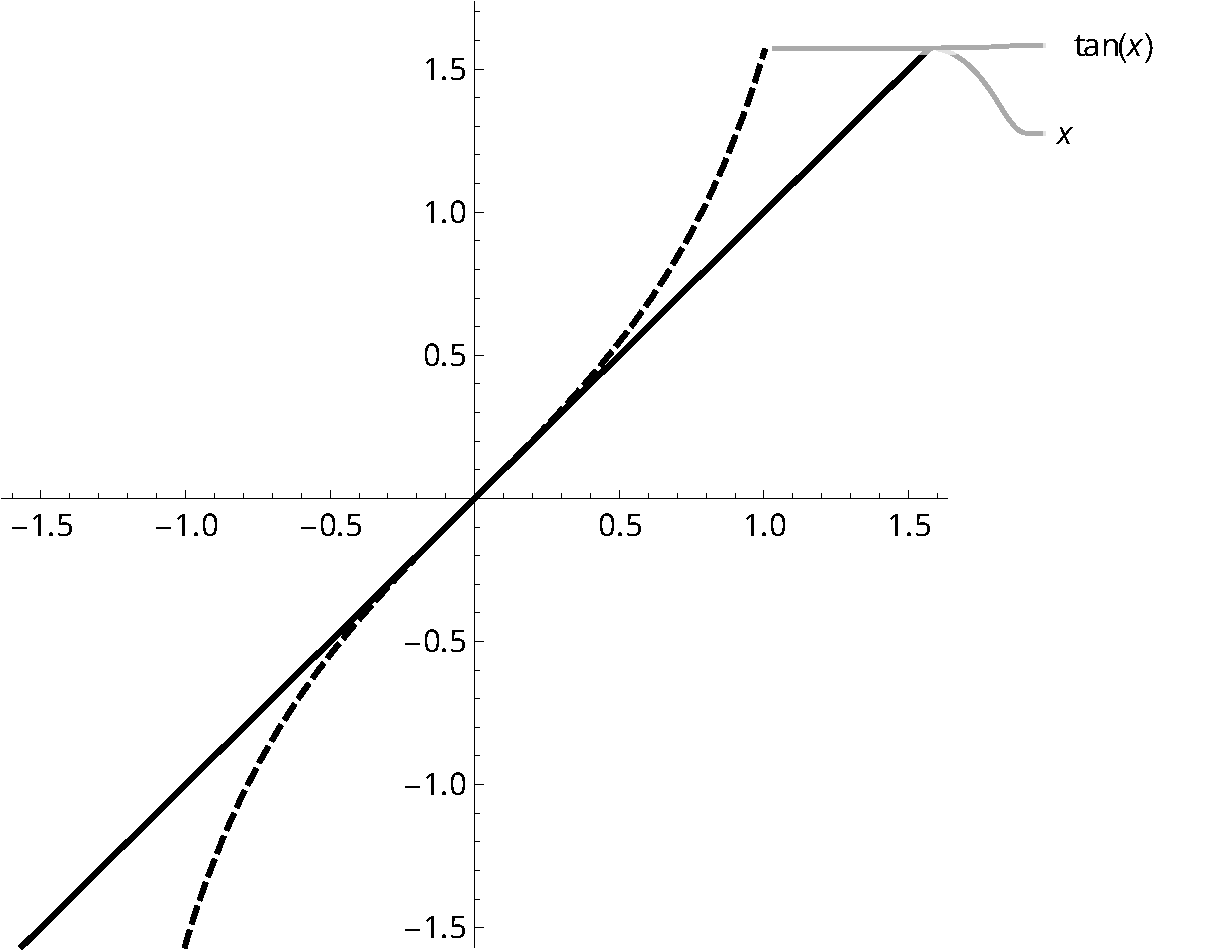
\includegraphics[width=0.5\textwidth]{figure/tanx-x.pdf}
    \caption{The figure of $\tan x$ and $x$, to illustrate $\tan x > x, x \in (0, \pi/2)$.}
    \label{fig:tanx-x}
\end{figure}

\section{定积分的应用}\label{app-finite-integral}

利用定积分定义求极限请参见
Section \ref{use-squeeze-or-definition-of-integral}.

其他定积分的应用请参考
\cite[page 435]{stewart}等参考书.

\section{无界函数反常积分}

\begin{definition}
    若函数 $f(x)$ 在点 $a$ 的任一邻域内都无界,
    那么点 $a$ 称为函数 $f(x)$ 的瑕点。
\end{definition}

\begin{theorem}[比较判别法]
    \label{comparasion-deterministic-informal-integral}
    设$f(x), g(x)$ 在$(a, b]$ 上连续,且
    $0 \leq f(x) \leq g(x)$,$x = a$ 为 $f(x)$ 和 $g(x)$ 的瑕点,则
    \begin{gather*}
        \int_a^b g(x) \mathrm dx \, \mbox{收敛} \Rightarrow \int_a^b f(x) \mathrm dx \, \mbox{收敛} \\
        \int_a^b g(x) \mathrm dx \, \mbox{发散} \Rightarrow \int_a^b f(x) \mathrm dx \, \mbox{发散} 
    \end{gather*}
\end{theorem}

\begin{theorem}[比较判别法的极限形式]
    \label{comparasion-deterministic-informal-integral-limit-form}
    设 $f(x), g(x)$ 在 $(a, b]$ 上非负连续,且
    \[
        \lim_{x \to a^+} \dfrac{f(x)}{g(x)} = \lambda \quad \mbox{(有限或无穷)}
    \]
    则
    \begin{align*}
        \int_a^b f(x) \mathrm dx \mbox{收敛} 
        \Leftrightarrow 
        \int_a^b g(x) \mathrm dx \mbox{收敛} &, \lambda \neq 0 \\
        \int_a^b g(x) \mathrm dx \mbox{收敛} 
        \Rightarrow 
        \int_a^b f(x) \mathrm dx \mbox{收敛} &, \lambda = 0 \\
        \int_a^b g(x) \mathrm dx \mbox{发散} 
        \Rightarrow 
        \int_a^b f(x) \mathrm dx \mbox{发散} &, \lambda = 0
    \end{align*}
\end{theorem}

\begin{corollary}[P积分]
    \label{P-integral}
    \[
        \int_a^b \dfrac{1}{(x - a)^p} \mathrm dx 
        \begin{dcases*}
            \mbox{收敛} & p < 1, \\
            \mbox{发散} & p \leq 1;
        \end{dcases*}
    \]
    \[
        \int_a^b \dfrac{1}{(b - x)^p} \mathrm dx 
        \begin{dcases*}
            \mbox{收敛} & p < 1, \\
            \mbox{发散} & p \leq 1.
        \end{dcases*}
    \]
\end{corollary}

